% mn2esample.tex
%
% v2.1 released 22nd May 2002 (G. Hutton)
%
% The mnsample.tex file has been amended to highlight the proper use of
% LaTeX2e code with the class file and using natbib cross-referencing.
% These changes do not reflect the original paper by A. V. Raveendran.
%
% Previous versions of this sample document were compatible with the LaTeX
% 2.09 style file mn.sty v1.2 released 5th September 1994 (M. Reed) v1.1
% released 18th July 1994 v1.0 released 28th January 1994

\documentclass[letterpaper,useAMS,usenatbib]{"mn2e"}
%\documentclass[letterpaper,useAMS]{"mn2e"}
%LINUX version of the path
%\documentclass[useAMS,usenatbib,letterpaper]{"/media/blank/Macintosh
%HD/Users/karenyng/Library/texmf/tex/latex/commonstuff/mn2e"}

% If your system does not have the AMS fonts version 2.0 installed, then
% remove the useAMS option.
%
% useAMS allows you to obtain upright Greek characters.  e.g. \umu, \upi
% etc.  See the section on "Upright Greek characters" in this guide for
% further information.
%
% If you are using AMS 2.0 fonts, bold math letters/symbols are available
% at a larger range of sizes for NFSS release 1 and 2 (using \boldmath or
% preferably \bmath).
%
% The usenatbib command allows the use of Patrick Daly's natbib.sty for
% cross-referencing.
%
% If you wish to typeset the paper in Times font (if you do not have the
% PostScript Type 1 Computer Modern fonts you will need to do this to get
% smoother fonts in a PDF file) then uncomment the next line 
%\usepackage{Times}

%%%%% AUTHORS - PLACE YOUR OWN MACROS HERE %%%%%
\usepackage{hyperref}
\usepackage{amssymb}
\usepackage{graphicx}
\usepackage{amsmath}
\usepackage[amssymb]{SIunits} 
\usepackage{booktabs}
\usepackage{hhline}
\usepackage{breqn}
\usepackage{standalone}
\usepackage{dcolumn}
	\newcolumntype{d}[1]{D{.}{.}{#1}}
\usepackage{tabularx}
\usepackage{booktabs}
\graphicspath{{graphics/}}
\newcommand{\mc}[1]{\multicolumn{1}{c}{#1}} % handy shortcut macro
%-----------------------------------------------------------------------

\defcitealias{D13}{D13}
\defcitealias{Jee13}{J13}
\defcitealias{M12}{M12}
\defcitealias{Sifon13}{Sif\'{o}n 2013}
\def\apjl{ApJL }
\def\aj{AJ }
\def\apj{ApJ }
\def\pasp{PASP }
\def\spie{SPIE }
\def\apjs{ApJS }
\def\araa{ARAA }
\def\aap{A\&A }
\def\nat{Nature }
\def\mnras{MNRAS }
\def\mnrasl{MNRASL }
\providecommand{\eprint}[1]{\href{http://arxiv.org/abs/#1}{#1}}
\providecommand{\adsurl}[1]{\href{#1}{ADS}}
\providecommand{\ISBN}[1]{\href{http://cosmologist.info/ISBN/#1}{ISBN: #1}} 


%-----------------------------------------------------------------------
\title[The dynamics and merging scenario of ACT-CL
J0102-4915, El Gordo]{The dynamics and merging scenario of the galaxy cluster 
ACT-CL J0102-4915, 
El Gordo}
\author[K. Y. Ng et al.]{K. Y. Ng$^{1}$, W. A. Dawson$^{2}$, D. Wittman$^{1}$, J.
Jee$^{1}$, J. Hughes$^{3}$, F. Menanteau$^{3}$, C. Sif\'{o}n$^{4}$\\
(temporary order)\\
$^{1}$Department of Physics, University of California Davis, One Shields
Avenue, Davis, CA 95616, USA\\ 
$^{2}$Lawrence Livermore National Laboratory, P.O. Box 808, Livermore, CA
94551-0808, USA \\
$^3$Department of Physics \& Astronomy,
Rutgers University, 136 Frelinghysen Rd., Piscataway, NJ 08854, USA\\
$^{4}$Leiden Observatory, Leiden University, PO Box 9513, NL-2300 RA
Leiden, Netherlands\\}

\begin{document}
%%---------to adjust for the weird bottom margin-----------
%\voffset=-.8in \hoffset=.15in
\date{arXiV 666} \pagerange{\pageref{firstpage}--\pageref{lastpage}}
\pubyear{1988} \maketitle \label{firstpage}
%-----------------------------------------------------------------------
\begin{abstract} 
    
Merging galaxy clusters with radio relics provide rare insights to the merger
dynamics as the relics are created by the
violent merger process. 

From the double radio relic observation and X-ray wake morphology, 
it is believed that El Gordo is observed shortly after the first passage
before reaching apo

We demonstrate one of the first uses of the
properties of the radio relic
to reduce the uncertainties of the dynamical variables 
and 3D configurations of a cluster merger, ACT-CL J0102-4915, El Gordo. 
At a redshift of 0.87, El Gordo (M$_{200c} = 
2.75\times10^{15} \pm^{7.4}_{1.5}$ M$_{\sun}$) is one of the most massive
clusters discovered in the early universe. The two subclusters of El
Gordo has a mass ratio of around 2:1. 
The X-ray and weak-lensing data of El Gordo show an offset of X kpc between
the intercluster gas and the dark matter (DM) at $\sim$4 $\sigma$ level.
All these features of El Gordo make it part of a valuable class of
dissociative mergers that can probe the self-interaction of dark matter.
%As more and more cluster mergers are being discovered using
%the radio relic emission detected in upcoming large scale radio surveys,
We employ a Monte Carlo simulation to investigate the three-dimensional (3D)
configuration and dynamics of El Gordo. 
We give a summary of the inferred
dynamical variables. By making use the polarization, velocity and position
of the radio relic, we are able to confirm at X $\sigma$ that the subclusters of El Gordo are moving away from each other. We find that
the 3D merger speed of El Gordo to be $\sim3000~\kilo\meter~
\second^{-1}$ (or in projected velocity = ), which is still consistent with the low line-of-sight
velocity of $\sim600~\kilo\meter~\second^{-1}$ based on the inferred time-since-collision ($TSC$ = Gyrs) and
the projection angle (\(\alpha = 41^{\circ}\pm \)). We put our estimates of $TSC$ and $\alpha$ into context by relating them to existing observations of El Gordo. 
Finally, we compare our simulation result of El Gordo to the simulation
result of the Bullet Cluster, and show that
El Gordo is a very promising candidate for giving tigher constraint than
the Bullet Cluster on the self-interaction of dark matter. 
(200 words)
(check against astro-ph word limit)
%\textbf{Findings}\\ 
%We found that the merger speed at the collision of El Gordo
%($\mathrm{km/s}$) is higher than those of the Bullet Cluster.  

%We estimate El Gordo to have a slightly higher TSC than the bullet cluster
%using the same analysis by Dawson (2012).  
%To be continued.  (250 words) 

\end{abstract}
%-----------------------------------------------------------------------
\begin{keywords}
gravitational lensing -- dark matter -- cosmology: observations -- X-rays:
galaxies: clusters -- galaxies: clusters: individual (ACT-CL J0102-4915) --
galaxies: high redshift 
\end{keywords}

%-----------------------------------------------------------------------
\section{Introduction} 
(NOT READY FOR PRIME TIME)
%\textbf{background - why do merging clusters of
%galaxies are worthy of investigating}
%Clusters of galaxies are some of the most interesting astrophysical
%laboratories. The environment of the cluster affects the evolution of the
%galaxy members. Redder galaxies are located closer to the dynamical
%centers of galaxies while bluer star-forming galaxies are located at the
%edge of clusters.

%----------------------------------------------------------------------
% To do:
% - make sure that when introduce the 2 subclusters - talk about the 
%   NW and SE notation
% - add Williamson 's paper as one of the reference for the first mention
%   of El Gordo
% - need citation for the estimated spectroscopic redshift of El Gordo
%----------------------------------------------------------------------

%\textbf{to motivate why we want to do this study} 
Mergers of dark-matter-dominated galaxy clusters probes properties
of the cluster components like no other systems. 
Clusters of galaxies are made up of 80\% of dark matter in mass content, 
with a smaller  portion of intercluster gas($\sim 15\%$ in mass content), and
sparsely spaced galaxies ($\sim 2\%$ in mass content) (REF). During a merger of
clusters, the subclusters are accelerated to high speeds of several
thousand \kilo \meter~\second$^{-1}$. The offsets of different components
of the subclusters dissociate show how various interactions of the different
components are at work. Observables such as offset between dark
matter and the other components may suggest dark matter self-interaction
(REF).  (The following sentence does not actually fit in this paragraph and
I have to put it somewhere else) difference of the galaxy colors in a merging cluster from relaxed cluster can also verify effects of environment on galaxy evolution.\par
%\textbf{background of El Gordo}
%\textbf{What literature exists for El Gordo.}

%van Weeren 2011a suggests that the double radio relic can provide clue to
%collisional parameters ???
Ever since the discovery of El Gordo in the Atacama Camera Telescope (ACT)
survey (REF), there is an ongoing effort for collecting comprehensive data
for El Gordo.
The presence of the radio relic, in
conjunction with a depression in the X-ray surface brightness shown in M12,
strongly suggest that El Gordo is a post-collision system so we limit our
discussion to inferring the time-since-collision. 

From the spectroscopy and Dressler-Schecter test for the member galaxies  in Sif\'{o}n et al. (2013), El Gordo is confirmed to be a binary merger 
without significant substructures. This picture is further supported by the
weak lensing analysis by Jee et al. (2013). The weak lensing analysis shows
a mass ratio of $\sim$2:1  between the two main subclusters, named according to their location as the northeast (NW) and southeast (SE) subclusters respectively. 
(See Figure \ref{fig:config}). El Gordo has interesting intracluster medium morphology as shown in the X-ray. In the northwest, it shows a wake feature, i.e.,
depression in the X-ray emissivity, while in the southeast, it shows
highest X-ray emissivity indicative of a cold gas core southeast of the
wake. The cold gas core may have passed from the northwest to the southwest
to have caused this morphology (Menanteau et al. 2011, hereafter M12). 
The extended mass distribution of El Gordo also makes it a good
gravitational lens. Zitrin et al. (2013) have found multiple strong
gravitationally lensed images around the center region of El Gordo. 
On the outer skirt of El Gordo, strong radio emission is detected in
the NW and the SE respectively. These radio emission has steep spectral
index gradient and are identified as radio relic created from a merger.\par 
%\begin{itemize}
%\item explains the 2D configuration of El Gordo - bimodal
%\item evidence that it is a merger 
%goes along a line joining northwest to southeast. 
%\item explains the spectroscopic surveys which confirms that that there are
%not a lot of line of sight substructures and that the line-of-sight
%velocity difference of the  
%\item strong lensing - many many arcs and elongated lens weak-lensing -
%bimodal distribution of matter  (describes what data has been available for 
%El Gordo) Since the
%discovery, an abundance of multi-wavelength data of El Gordo has been
%analyzed according to the two-dimensional projected view. \par 
%\item explain the wake feature (depression in X-ray) and the cold core in
%the SE which has high X-ray emission and point out it shows a recent merger 
%unlike the bullet cluster, El Gordo lacks a prominent X-ray shock
%\end{itemize}\par
%\textbf{Explains the importance of radio relic in constraining the merger
%physics.} Radio relics are direct products of the merger process itself.
%
%\begin{itemize}
%
%\item explains the double radio relic and their formation
%synchrontron emission in the radio wavelength with steep falloff of
%spectral indices.
%\item explains compression of magnetic field would cause polarization
%signal perpendicular to the merger axis 
%\item explains the current status of simulations in understanding radio
%relic
%\item  
%\end{itemize}
\begin{figure}
	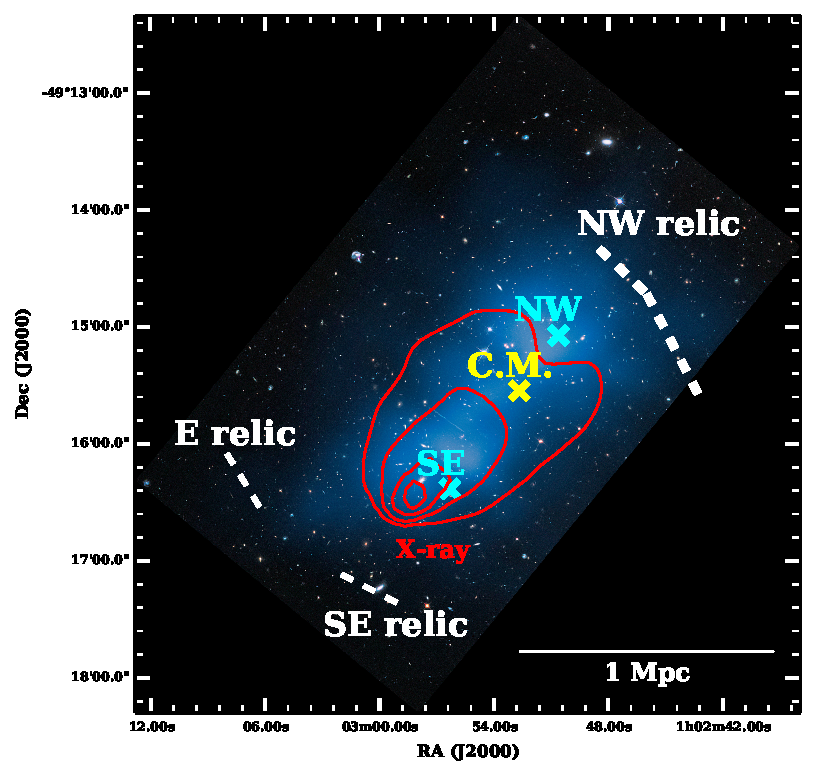
\includegraphics[width=\linewidth]{ElGordo.pdf}
	\caption{Configuration of El Gordo (to decide which figure to use,
	this one is from Lindner et al.) \label{fig:config}}
\end{figure}
El Gordo is one of small sample of galaxy clusters ($\sim 50$) that have
been associated with a radio relic. (This paragraph needs a lot more
organization) Even fewer of them have been studied in
great details, making El Gordo a valuable candidate for further analysis. 
%Cosmological simulations have largely complement the studies of the
%observed radio relics.  
%The study of radio relics is just taking off. 
%Cosmological
%simulations have also been employed to study the properties of the radio
%relics. (explain how both observations and simulations confirm radio relics
%are due to a cluster merger and that double relics are proposed to
%correspond to binary mergers)
%Radio relic, also known as radio shockwaves, are created during the violent
%merger of clusters of galaxies (See Ensslin's paper for a review of the
%physics). 
%Such double radio relics are also exhibited in other confirmed merging clusters of galaxies, such as REF missing etc. 
%
%(more description of how the paper comes up with emission in their simulations)
%
%\textbf{(Need to add transition from background to this paragraph to
%motivate why we have to study El Gordo) 
Furthermore, El Gordo satisfies the four criteria for being a dissociative merger which are proposed to be excellent
probes of self-interacting dark matter (Dawson et al. 2012) . (1) The subclusters
of El Gordo has a small ratio of mass, i.e. $\sim 2:1$ (Jee et al. 2013,
hereafter J13). (2) The merger axis, the line joining the two subclusters,
coincides with the alignment of the double radio relic propagating outward at the periphery of the cluster (Menauteau et al. 2012,
hereafter M12). This suggests a simple merger configuration with small
impact variables.  (3) The X-ray luminosity peak is shown to be offset
from the weak-lensing peak by X kpc at X $\sigma$ level (J13). (4) The
observation of the double radio relic suggests that the angle between the
merger axis and the plane of the sky has to be reasonably small (M12,
Lindner et al. 2013), or else
the relic may appear as a halo instead. \citep{S13} \par 


%\textbf{motivation} 
%\textbf{summarizes what is missing for the understanding of the merger of El
%Gordo, which is the projection angle and the time-since-collision.}
In this paper, we perform results of simulations for modeling the time
evolution of the mergers. 
Determining the time-since-collision of mergers of similar clusters helps
us reconstruct different stages of a cluster merger.
Mergers of clusters proceed on the time-scale of millions of year,
observations of each cluster only provides a snapshot of a particular type
of merger. In order to understand the merger process observationally, 
we need to capture
and identify different stages of similar dissociative mergers. \par 

Another crucial piece of missing information is the 3D
configuration, i.e. the projection angle $\alpha$, which contributes the
largest amount of uncertainties to the dynamical variables \citep{D13}.
With a large projection angle $\alpha$, the radio emission may appear as a
radio halo instead.  \citep{S13}\par 
%\textbf{motivation2}
This work is particularly important since it is forbiddingly
expensive to simulate clusters similar to El Gordo in high resolution. 
The probability for finding an analog of El Gordo in a cosmological
simulation is as low as \% \citepalias{M12}. A realistic cosmological simulation of
El Gordo is thus computationally expensive. Under the hierarchical picture
of structure formation in the $\Lambda$CDM model, there is a rare
chance for massive clusters like El Gordo to have formed at a redshift of
$z = 0.87$.  Staged simulation would not be able to probe the angular
dependence. 
Both weak lensing analysis and BLAH DATA of El Gordo \citep{Jee13} has revealed a
relatively simple bimodal mass distribution.  The lack of complex
substructures makes modeling of El Gordo with only two subclusters possible.

\par

In this paper, we adopt the following conventions: (1) we
assume the standard $\Lambda$CDM cosmology with $\Omega_{m} = 0.3$, $\Omega_{\Lambda} = 0.7$. (2) All confidence intervals are quoted at the 68\% level unless otherwise stated. 
(3) All credible intervals (a.k.a. Bayesian confidence intervals that also
takes into account prior probability) are also
quoted at the 68\% level unless otherwise stated and are central credible
intervals. (4) All quoted masses ($M_{200c}$) are based on mass contained
within $r_{200}$ where the mass density is 200 times the critical density
of the universe ($\rho_{crit}$) at the redshift of $z = 0.87$. 
%(5) We
%demonstrate that the application of a uniform sampling PDFs derived due to the
%integrated polarization fraction of the radio relic does not introduce
%large biases into our estimators in section \ref{sec:relic}, and unless
%otherwise stated, the simulation results we quote are those after applying
%the uniform radio relic filter.  \par 

%-----------------------------------------------------------------------
\section{DATA}
\input{2.0_data_section.tex}
\section{METHOD -- Monte Carlo simulation} 
For this analysis, we made use of the collisionless 
dark-matter-only Monte Carlo modeling code written by Dawson (2013),
hereafter \citepalias{D13}.  
In the code, the time evolution of the head-on merger was computed
analytically, assuming that the only dominant force is the gravitational attraction from
the masses of two truncated Naverro-Frenk-White (hereafter NFW) DM halos.
Other major assumptions for modeling systems with this code include
negligible impact parameter and no self-interaction of dark matter.\par

In the Monte Carlo simulation, many realizations of the collision is
computed from the inputs of each realization, including
the data ($\vec{D}$) and the model variable ($\alpha$). In particular,
the standard required data, which were in the form of samples of the probability density
functions (PDFs), included the masses ($M_{200_{NW}},M_{200_{SE}}$) the
redshifts ($z_{NW}, z_{SE}$) and the projected separation of the two
subclusters ($d_{proj}$).  
%For the $j-$th realization, w
In each realization, we randomly drew the samples of the PDFs.
%
%\begin{equation}
%	D_i^{j} \sim \mathcal{L}(\vec{\theta}|D_i) =  P(D_i | \vec{\theta})
%\end{equation}
%and we also draw the model variable $\alpha$ from the prior:
%\begin{equation}
%	\alpha^j \sim P(\alpha)
%\end{equation}
These inputs are then used for computing the output variables
($\vec{\theta}^\prime$) by making use of conservation of energy to describe
their collision due to the mutual gravitational attraction.
%\begin{equation}
%(\vec{\theta}^\prime)^{(j)} = f(\vec{D_i}^j, \alpha^j) 
%\end{equation}
%where $f$ are some suitable functions expressing the conservation of energy.
(See Table \ref{tab:inputs}
for quantitative descriptions of the sample PDFs and we outline how those
PDFs are obtained in the following subsections.) 
To ensure convergence of the output PDFs, in total, 2 million (to be
confirmed) realizations were computed. The results, however, are
consistent up to a fraction of a percent just from 20 000 runs
\citepalias{D13}.\par    
We note that the Monte Carlo simulation is written under a Bayesian
framework but differs from conventional Bayesian inference. The Bayes
chain rule underlies the simulation is:
\begin{equation}
    P(\vec{\theta}|\vec{D}) \propto P(\vec{D}|\vec{\theta})P(\vec{\theta})
\end{equation}
where the likelihood is defined to be the PDF of $\vec{D}$ given $\vec{\theta}$,
i.e. the input variables, not statistical parameters, and the priors are
defined to be the probabilities due to prior knowledge of the estimated values of
$\vec{\theta}$. The output variables $\vec{\theta}^\prime$, on the other
hand, were computed according to the conservation of energy, which is represented by a suitable
function form $f$ below. For example,the calculation of the $j$-th realization: 
\begin{equation}
    (\vec{\theta}^\prime)^{(j)} = f(\vec{\theta}^{(j)}, \vec{D}) 
\end{equation}    
The estimated values of $(\vec{\theta}^\prime)^{(j)}$ were then computed
over all $j$ realizations. Finally, we took physical
constraints on $\vec{\theta}$ and $\vec{\theta}^\prime$ into account by
excluding the unphysical realizations, and we refer to this process as
``applying prior probability''. 

%To model projection effects, we randomly draw a projection
%angle in each realization. We throw out realizations with unphysical
%outputs.  \textbf{what are the inputs}


\subsection{Inputs of the Monte Carlo simulation}
\label{sec: inputs}
\setcounter{table}{0} 
\begin{table} 
\caption{Properties of the sampling PDFs of the Monte Carlo simulation }  
\begin{center} 
\begin{tabular}{@{}lcccc}
\hline Data & Units & $\mu$ & $\sigma$ & Ref\\ \hline
$M_{200c_{\mathrm{NW}}}$ & $10^{14}$ M$_{\odot}$ & & & \citetalias{Jee13}\\ 
c$_{\mathrm{NW}}$ & / & & & \citetalias{Jee13} \\ 
$M_{200c_{\mathrm{SE}}}$ & $10^{14}$ M$_{\odot}$ & & & \citetalias{Jee13}\\
$c_{\mathrm{SE}}$ & / & & & \citetalias{Jee13}\\ 
$z_{\mathrm{NW}}$ & / & 0.86901 & 0.00017$^b$  & \citetalias{M11},
\citetalias{Sifon13}\\
$z_{\mathrm{SE}}$ & / & 0.87175 & 0.00019$^b$  & \citetalias{M11},
\citetalias{Sifon13}\\ 
d$_{\mathrm{proj}}$ & Mpc & & & \citetalias{Jee13} \\ 
\hline
\end{tabular} 
\end{center} 
\label{tab:inputs} 
\footnotesize{
$^a$This $\sigma$ corresponds to the $68\%$ central Bayesian
credible interval computed from the posterior probability of our MCMC
analysis.\\
$^b$This $\sigma$ corresponds to the biweight scale. \\
$^c$We use the full PDFs as the inputs of our simulation so
different ways of denoting the uncertainties do not affect the simulation.\\ 
%\textbf{References:} (1) Jee et al. 2013 (2) Menanteau et al. 2011}
}
\end{table}


%-----------------------------------------------------------------------
\subsubsection{Membership selection and redshift estimation of subclusters}
% \textbf{how do we determine the overall membership}
% relevant info of the membership is in M11 table 1
% cannot determine the membership of two galaxies 
% spatial cut is defined in M11 p.9 first paragraph 

% paragraphs needs to be reorganized 
We adopt the identification of galaxy membership of El Gordo given by
\citepalias{M11} with a total count of 89 galaxies.
%The overall membership of the galaxies
%of El Gordo was first determined using a shifting gapper method
%\citep{Fadda96} after applying a rest frame cut of
%4000~\kilo\meter~\second$^{-1}$ \citep{Sifon13}. This method gives a
To further distinguish member galaxies of each subcluster, we adopt a
redshift cut of $z < 0.886$, and a spatial cut approximately perpendicular
to the 2D merger axis from \citetalias{M11} to determine that
there are 51 members in the NW subclusters and 35 members in the SE subclusters (See Figure
\ref{fig:membership}). 
The spatial cut indicated by the green line was done after
mapping the world coordinates to pixel coordinates to avoid anamorphic distortion. 

%Compare and contrast the amount of bootstrapping and the reported
%redshifts and velocity dispersion.
After identifying members of each subcluster, we performed 10, 000 bootstrap realizations to estimate the biweight
locations of the redshifts of the respective members in order to obtain the
samples of the PDFs of the redshifts of each subcluster. 
The spectroscopic redshift of the subclusters were
determined to be 
%$z_{total} = \pm $ 
$z_{\mathrm{NW}} = 0.86842 \pm 0.0011$ and 
$z_{\mathrm{SE}} = 0.87131 \pm 0.0012$, where the quoted numbers represent the
biweight location and 1$\sigma$ biased corrected confidence level
respectively \citep{Beers90}.  
%These biweight location estimators are less susceptible to outliers than
%the mean and standard deviations. 
Both the estimated redshifts of the subclusters and the uncertainties are
consistent with estimates given by \citealt{Sifon13}, and the fact that El
Gordo shows large velocity dispersion and has the largest velocity
dispersion among all the ACT galaxy clusters as reported by
\citetalias{M13}. These redshifts of the subclusters correspond to a
radial velocity difference in the frame of the NW subcluster
to be $476 \pm 242 $ km/s. We estimate the radial velocity differences of the
subclusters by first calculating the velocity of each subcluster with
respective to us, using  
\begin{equation}
	v_i = \left[ \frac{(1+z_i)^2 - 1 }{(1+z_i)^2 + 1 }\right]c
\end{equation}
where $c$ is the speed of light. And then the radial velocity was calculated
by: 
\begin{equation}
	\Delta v_{rad}(t_{obs}) = \frac{|v_2 - v_1|}{1-\frac{v_1 v_2}{c^2}}
\end{equation}
This result is lower than the the quoted radial velocity differences of
$586$
km/s reported by \citetalias{M11} from the approximation of $\Delta v_{rad}
= c(z_1 - z_2) / (1 + z_1)$ in the frame of the NW subcluster. 


\begin{figure}
	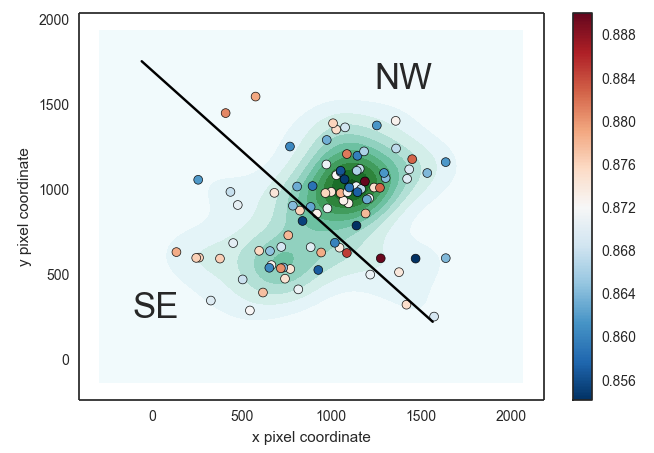
\includegraphics[width = \linewidth]{confirmed_member_divide.png}
	\caption{\label{fig:membership} The division of
the member galaxies among the two subclusters of El Gordo by a spatial cut
(green line). The color bar shows the color mapping of the spectroscopic
redshift of the member galaxies, with the redder end indicating higher
redshift.} 
\end{figure}

%We confirm the existence of the subclusters of El Gordo from the 2D spatial
%location of the galaxies, with the more massive cluster lying in the
%northwest (NW) and the less massive subcluster lying in the southeast(SE)  (REF - also have to reference the other literature
%for confirmation in the other wavelengths)
%
%Specifically, the membership of the NW and SE subclusters are
%determined based on a combination of the redshift and the spatial location. 


\begin{figure}
	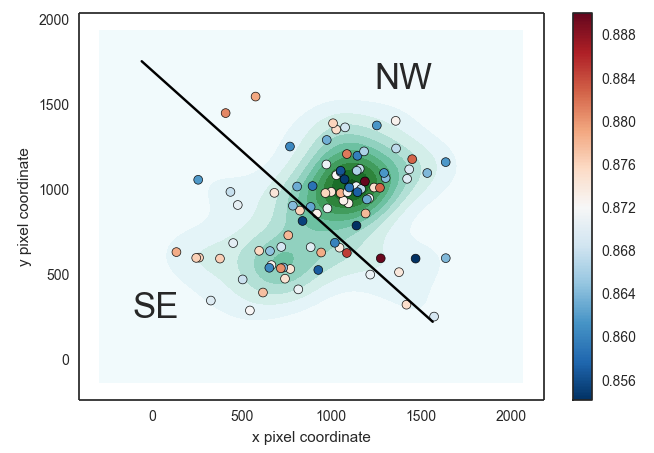
\includegraphics[width = \linewidth]{confirmed_member_divide.png}
	\caption{\label{fig:membership} The division of
the member galaxies among the two subclusters of El Gordo by a spatial cut
(green line). 
The color bar shows the color mapping of the spectroscopic redshift of the
member galaxies.} 
\end{figure}

%-----------------------------------------------------------------------
\subsubsection{Weak lensing mass estimation} 

%The input 
We obtained the PDFs of the masses of the subclusters by doing a Monte
Carlo Markov Chain (MCMC) analysis of the reduced shear from the
weakly lensed background galaxies similar to \citet{Dawson12}. We computed the reduced shear signal
generated by two NFW halos according to \citet{Umetsu10} (See Appendix
\ref{app:MCMC} for
details of implementation and output diagnostics).
At each step we followed the procedure of a
Metropolis algorithm.  The transition kernel was set to
be the log likelihood of fit of the model shear to the reduced shear of the
data (\ref{eqn:jointposterior}).
In total, eight MCMC chains were used. After every 5000 MCMC steps for all
the chains, we computed the R coefficient \citep{Gelman92}  to
check for convergence. We performed more MCMC steps as long as convergence
was not achieved. After convergence was achieved, we removed the
burn-in portions of the MCMC chains and used the resulting MCMC chains as
samples of the PDFs of the masses. \par 
% this is from Jee13 section 3.5
We make use of an effective redshift of $z_{\text{eff}} = 1.37$ or $\beta
= 0.276$ \citepalias{Jee13} and $g' \approx (1 + 0.79 \kappa)~g$ \citepalias{Jee13}
and \citep{Seitz97}.    
%\textbf{The inputs of our MCMC mass inference are from proposal blah,
%which is similar to \citepalias{Jee13}, however, this
%separate implementation of the MCMC analysis code is different than
%\citepalias{Jee13}.} 
We used a catalog of reduced and bias-corrected background 
galaxy shapes from Hubble Space Telescope PROP 12755, and these galaxies
were discussed as the population in Region A in
\citetalias{Jee13}. (! \citealt{Jee13} actually used
additional data) On the other hand, we fixed the
position of the centers of the NFW halos to be  the luminosity peaks of the
respective galaxy populations of  the two subclusters, which are at R.A. $=
01$:02:51.68, Decl. = $-49$:15:04.40 and R.A. = $01$:02:38.38, Decl. =
$-49$:16:37.64 for the NW and SE subclusters
respectively \citepalias{Jee13}. (! Lori and Nick actually asked why we do not free
the centroids like Jee 13)  The agreement between our analysis and \citepalias{Jee13} to within
the 68\% credible interval serves as a sanity check on the estimated masses. 
%Other sanity check including the control of acceptance rate between 20\%
%and 50\%. 

The mass estimates from \citealt{Jee13} are $M_{200c} = 13.8 \pm
2.2 \times 10^{14}~h_{70}^{-1} M_{\sun}$ for the NW subcluster and $ M_{200c} = 7.8 \pm
2.0 \times 10^{14}~h_{70}^{-1} M_{\sun}$ for the SE subcluster. 


%----------------------------------------------------------------------

\subsubsection{Estimation of projected separation ($d_{proj}$) } 
To be consistent with our MCMC mass inference, our Monte Carlo simulation takes 
the projected separation of the NFW halos to be those of the two aforementioned 
luminosity peaks.
%A iterative centroiding method is used to find the centers of the two
%subclusters of El Gordo.

\subsection{Outputs of the Monte Carlo simulation}
\label{sec: outputs}
We outline the outputs of the simulation here to facilitate the discussion
of the design of the priors used in the simulation. The simulation
provides PDF estimates for many of the output variables. Variables
of the most interest include the time dependence and $\alpha$, which is
defined to be the projection angle between the plane of the sky and the merger axis. Other output variables are dependent on $\alpha$ and the time
dependence. Specifically, the simulation denotes the time dependence by
providing several characteristic time-scales, including the time
elapsed between the collision and when the subclusters first reach apoapsis
($T$) and the time-since-collision.  

The two versions of the time-since-collision variables $TSC_0$ and
$TSC_1$ denotes different possible merger scenarios. 1) We call the scenario for which the subclusters are
moving apart after collision to be ``outgoing" and it corresponds to the
smaller $TSC_0$ value, and 2) we call the alternative scenario 
``returning" for which the subclusters are approaching each other after turning
around from the apoapsis for the first time and it corresponds to $TSC_1$.
We describe how we use to break the degeneracies of the two scenarios in
section \ref{sec: positionprior}. 
 
The simulation also output estimates of variables that characterize
the dynamics of the merger. The 3D velocities, both at the time of the
collision ($v_{3D}(t_{col})$) and at the time of observation
($v_{3D}(t_{obs})$) are provided. The maximum 3D separation ($d_{max}$),
which is defined to be the distance between the position of collision to
the apoapsis, is also part of
the outputs. (See the lower half of Table \ref{tab:outputs} for all the outputs).
%Here we present results based on:\\  %1) a flat radio prior\\
%2) a uniform prior over a range of most likely 3D separations\\
%3) a Gaussian prior  
%We discuss in subsection \ref{sec:priors}  on the use of the default filters
%and two new filters designed according to the observed data and the physics of the radio relic.
%
%\textbf{While the underlying formalism of the Monte Carlo simulation is
%    based on the Bayes theorem, we caution the reader that this simulation
%    does not correspond to a conventional Bayesian parameter estimation but
%    more similar to the Bayesian uncertainty estimation method mentioned in Saltelli 
%    et al. (2004). (See appendix \ref{} for a more in-depth discussion)}



%-----------------------------------------------------------------------
\subsection{Design and application of priors} 
\label{sec:priors}
The strength of the Monte Carlo simulation by \citep(D13) is its ability
to detect and rule out extreme input values that would result in
unphysical realizations. 
Our default Monte Carlo filters are described in D13 and they are applied to ensure 
unphysical realizations in the simulation are ruled out. 
In addition to the default filters, we also examine the effects of applying 
two filters derived based on the position and the integrated polarization
fraction of the radio relic of El Gordo respectively. 
%(See Appendix \ref{tab:priors} for a complete list of filters used in this paper.) 

\textbf{El Gordo shows remarkable double radio relics on the periphery
(M11)} The radio relic  of El Gordo was first mentioned in the Sydney University
Molonglo Sky Survey (SUMSS) data in low resolution at 843 MHz
\cite{Mauch03} as shown in
M11. The higher resolution radio observation conducted by \cite{L13} at 610
\mega Hz and 2.1 \giga Hz confirms that those radio emission correspond to
radio relic after removing effects of radio point sources.
%\begin{itemize}
%\item talks about the observable, which is the comoving kinetic power through each shock surface
%\item refer to diffussive shock acceleration (DSA) mechanism?
%\item Kang \& Jones treatment of Mach number-dependent efficiency
%considering the possibility of having an non-isotropic magnetic field  
%$KJ_BparallelRadial$ model
%\end{itemize}

Radio relics have been suggested to be able to constrain the
mass ratios, the projection and the merger configuration. (Cite one of Reinout's paper) 
Ever since the first detection of radio relic,cosmological hydrodynamical simulations of
merging clusters have been used to model their emission spectrum and
geometry. (Vazza et al. 2011, van Weeren and Bruggen 2011 et al., Bonafede
et al. 2013, En{\ss}lin et al. 1997, Br\"{u}ggen et al.,  Skillman et al.
2013) While such cosmological simulations have provided valuable insights
to verifying the physical models, they are expensive both in terms of
computational power and novel techniques have to be invented in order to
analyze the large amount of simulated data so progress has been slow. 
Our Monte Carlo simulation can make use of known physics combined with the
preliminary results from such cosmological simulations to use properties of
the radio relic to constrain merger dynamics. 
Compared to hydrodynamical simulations or cosmological simulations, this
    Monte Carlo simulation is not demanding in terms of CPU time, therefore, we
    can run many realizations in order to probe how the input variables
affect the output variables. 

%\begin{figure}
%	\includegraphics[width=\linewidth]{d_3d_prior1.png}
%	\caption{The marginalized output PDFs of the observed 3D separation
%		($d_{3D}$) 
%		with and without the radio prior applied. 
%		(maybe I should replot this more nicely without too many
%		distracting lines but only the lines showing the location)
%		%The vertical
%		%lines denote, dashed line: biweight location, dash-dot
%		%line: 68\% credible limit, dotted line: 95\% credible
%		%limit.
%	\label{fig:radioprior}}
%\end{figure}


%\subsubsection{Weighting function based on the observed position of the radio relic}\label{sec:relic} 
%-----------------------------------------------------------------------
%Among the known galaxy cluster mergers that are associated with radio
%relics, \cite{Vazza12} noted that most of them have radio relic located
%more than 800 \kilo pc away from the merger center. \cite{Vazza12} then
%conducted hydrodynamical simulations of twenty of known galaxy mergers with 
%radio relic to investigate this observed trend. They found a radial
%trend of kinetic power dissipation increasing up to around half the virial
%radius (r$_{vir}$) of the cluster. Summarizing the results from the proposed model for energy dissipation of the radio relic, \cite{Vazza12} gives the range of highest kinetic power emission in a range of 
%$.2 ~r_{\mathrm{vir}} < d_{\mathrm{3D}} < .5~r_{\mathrm{vir}}$.
%
%
%% In particular, Vazza et al. (2011) showed dependence of observed
%%location of radio relic: when the clusters are at small separation, the
%%Mach number is too high for a radio shock to form and the steep fall off of
%%the emission power of the radio relic as a function of separation makes it
%%difficult to observe a radio relic when it has propagated beyond a certain
%%separation.  
%
%%\textbf{We take into account the uncertainties of their modeling and 
%% construct prior probability on a range of 3D separation for which the kinetic
%%power dissipation of the radio relic is more than 10\% of the peak value.} 
%Since we do not have information on how the probability of
%being able to observe the relic would fall off as a function of emission power, we adopt a conservative approach and designed a uniform prior. 
%%and contrast that to a flat prior to test the effect of the prior on the output variables. 
%We also take into account the uncertainties of the different proposed power
%emission model and come up with a prior of:
%\[
% \text{P}({d_{3D}}) = 
%\begin{cases} 
%\text{constant,} & \text{for 1.0  Mpc} < d_{3D}(t_{\mathrm{obs}}) < 3.0 \text{ Mpc}\\
%0, & \text{otherwise}
%\end{cases}
%\]
% for El Gordo.\par 
%%\begin{equation}  
%%P(d_{3D}(t_{\mathrm{obs}})) = 
%%\begin{cases}
%%1/C, \text{ if }1.0 \text{ Mpc } < d_{3D}(t_{\mathrm{obs}}) < 3.0 \text{ Mpc} \\ 0, \text{ otherwise}
%%\end{cases}
%%\end{equation}
%
%\begin{figure}
%	\includegraphics[width=\linewidth]{alpha_pdf_prior_diff.png}
%	\caption{The projection angle with and without the radio relic
%prior applied. (Needs to update and label the figure better)} 
%\end{figure}

\begin{table*} 
\begin{minipage}{180mm} 
\caption{Table of the output PDF properties of the model variables and
output variables from Monte Carlo simulation
\label{tab:outputs}} 
\begin{tabular}{@{}lccccccc@{}}
\toprule 
&&&Default priors & & &Default + position priors  \\ 
\hline
Variables & Units & Location & 68$\%$ CI $^{\dagger}$ & 95$\%$ 
CI & Location & 68$\%$ CI  & 95$\%$ CI \\
\hline
$\alpha$ &(degree)&&&&&&\\ 
\hline
$TSC_0$&Gyr&&&&&&\\
$TSC_1$&Gyr&&&&&&\\
$T$&Gyr&&&&&&\\
$d_{max}$ &Mpc&&&&&&\\
$v_{3D}(t_{obs})$ & \kilo \meter~\second$^{-1}$ &&&&&&\\
$v_{3D}(t_{col})$ & \kilo \meter~\second$^{-1}$ &&&&&&\\
$d_{max}$ &Mpc&&&&&&\\
$d_{3D}$ &Mpc&&&&&&\\
\bottomrule 
\end{tabular} 
\footnotesize{\\$\dagger$ CI stands for credible interval} \\ 
\end{minipage} 
\end{table*} 


%---------------------------------------------------------------------------
\subsubsection{Monte Carlo priors based on the polarization fraction of the radio relic}
In particular, \cite{L13} reports an integrated
polarization fraction of $\sim33\%$ for the two identified relics. The
high integrated polarization fraction can be explained by uniformly aligned
magnetic field. (Synchrotron emission from unorganized magnetic field are
randomly polarized) We refer to a model from \citet{E98} with
the following physical picture: during a merger, the intracluster medium is compressed, this aligns the unordered
magnetic field perpendicular to the line joining the cluster center to the
radio relic. (\citealt{E98}, \citealt{vanWeeren10}, \citealt{Feretti12})
Thus, the synchrotron emission emitted from the electrons near this aligned
magnetic field is strongly polarized perpendicular to this magnetic field. \par
\textbf{The major assumption behind the design of our filter
is that the integrated polarization fraction is a monotonically
decreasing function of $\alpha$.} 
This assumption is inspired by the class of models given by \cite{E98}, 
which, despite various inputs for spectral indices and magnetic field strength, each predicts a monotonically decreasing integrated
polarization fraction as a function of $\alpha$. 
%This assumption is yet to be verified by cosmological simulations of radio relic. 
In particular, we refer to a model from \cite{E98} that would give the most
conservative estimate on the upper bound of $\alpha$. 
This model predicts a maximum integrated polarization fraction of
$\sim75\%$ when $\alpha = 0$ . From this model, the observed integrated
polarization fraction of 33\% corresponds to $\mu_\alpha =  39\degree$. 
%We consider 39\degree as an upper bound on the projection angle since this idealized model assume isotropic distribution of magnetic field and
%electrons. 
This  polarization fraction of $\sim 75\%$ predicted by \citep{E98} is
consistent with the upper bound of relic polarization fraction in cosmological
simulations \citep{S13}. No other model of the magnetic field should predict a higher polarization fraction, thus it is highly unlikely that we see 33\%
integrated polarization at $\alpha > 39\degree$. \par 
\textbf{We cannot rule out $\alpha \leq 39\degree$ as a result of possible
variations in the magnetic field.} \cite{E98} assumes an isotropic
distribution of electrons in an isotropic magnetic field. Cosmological
simulations of radio relics from \cite{S13} show varying polarization
fraction across and along the relic assuming $\alpha = 0$, resulting in a
lower integrated polarization fraction. 
%Due to these likely variations in the true magnetic field, the true observable integrated polarization values at a given $\alpha$ can be lower than what is predicted by \cite{E98}. 
%For example, it is possible that the radio relic of El Gordo has a lower maximum face-on polarization fraction than 75\%, but if we are viewing the relic at a smaller $\alpha$, the integrated
%polarization fraction can still comes out to be 33\%.
For example, it is possible to see a edge-on radio relic ($\alpha = 0$) with integrated polarization fraction of 33\%. 
\par 
%With simplifying assumptions, \cite{E98} have derived the integrated polarization fraction of a radio relic as a function of the viewing
%angle ($\delta = 90\degree - \alpha$).
% and the compression
%\~{R} of the magnetized region where the relic is generated. 
%. The simplifying assumptions, such as having an
%isotropic distribution of unshocked magnetic fields and electrons etc.,
%represents an idealized case showing maximum possible polarization fraction at a given $\alpha$.  
%% Cosmological simulations of radio
%relic \citep{S13} show a maximum integrated polarization fraction $\sim75\%$ at
%$\alpha = 0$ as predicted by \cite{E98}. 
%After accounting for different spectral
%indices and magnetic field strength, 
%The simplifying
%assumptions, such as having an isotropic distribution of unshocked fields
%and an isotropic distribution of electrons etc. \citep{E98}, gives
%polarization fraction as high as $\sim$ 75\% when $\alpha = 0$. 

%For an
%actual merger, the magnetic field can be less isotropic,  and the resulting polarization fraction at a given $\alpha$ would be lower. This postulate is backed up by the edge-on view of polarization fraction of simulated relics, such as the top left hand panel of figure 9 from Skillman et al. 2013.
%%This model, however, assumes an isotropic distribution of electrons in an isotropic magnetic field. \cite{E98}
%%These mathematical relationships underlies the design of this prior based on observed polarization fraction. The different cases that \cite{E98} considered have different magnetic field strengths and various spectral indices.
%We note that power of polarized synchrotron emission from relativistic electrons has a ratio of 7:1 between parallel polarization and perpendicular polarization. 
%Therefore,   
%
%\par
\textbf{Observation also introduces uncertainties that we have to take into account}. \cite{S13} shows that after convolving the
simulated polarization signal with a Gaussian kernel of 4\arcmin to match
observable resolution, the polarization fraction drops to between 30\% to
65\% even when $\alpha = 0$. 
Other uncertainties come from the fact that the inferred spectral indices
differ between the two observed frequencies and vary between the three
identified relic sources \citep{L13}. 
%\textbf{We pick a form of uniform prior, to represent
%the uncertainties in both the modeling (\citealt{E98}, \citealt{S13}) and the interpretation of the data from \cite{L13}.} 
Following previous discussion, we pick a value of $\mu_\alpha =39\degree +
2 \degree$ to filter realizations, i.e. we do not draw values of $\alpha >
41\degree$. The extra $2 \degree$ in the prior is included to account for the uncertainty of the integrated polarization fraction reported by \cite{L13}. 

%For the width of fall off of the sigmoidal function, we pick
%$\sigma_\alpha = 1\degree$ that corresponds to the uncertainty of the
%integrated polarization fraction reported by \cite{L13}.    

%\begin{itemize}
%\item spectral index of ...
%\item During the merger process, the hot intracluster is cluster merger compresses the magnetic field and orders the polarization.    
%\item \cite{L13} reported that the polarization can constrain viewing angle to be $> 18 \degree $-- check if this viewing angle is defined the same way 
%\item Ensslin 's work which is an application of the theory of
%plane-parallel shock acceleration, which can be justified by the large
%radius of the shock sphere
%\item we consider the most conservative constraint that can be recovered
%from this model, which is strong/weak field case with a spectral index of
%$\alpha_{\text{spectral}}\sim 2$ combined with the observed mean
%polarization fraction of $P \sim 33.3\%$, we recover a  
%\item
%\end{itemize}
%\begin{equation}
%P(\alpha) = 
%\frac{1}{2} - \frac{1}{2} \text{erf}\left(\frac{1}{\sqrt{2}}\frac{\alpha -
%(\mu_\alpha+3\degree)}{\sigma_\alpha}\right)  
%\label{eqn:prior}
%\end{equation}
%
%\noindent See Appendix \ref{app:priors} for a plot of (\ref{eqn:prior}).

%The polarization information has larger constraining power than the .   
%To test the effects of applying the prior on the aforementioned range of
%separation,  we have come up two priors and applied them separately
%%Therefore, the distance between the subclusters, which has to be less than twice the 3D distance between the radio relic from the center of the cluster, is taken conservatively to be $1.0~\mega$pc $<$ d$_{\mathrm{3D}}
%%(t_{\mathrm{obs}}) < 3.0~\mega$pc. 
% to the 3D separation of the subclusters at the time of observation 
%($d_{\mathrm{3D}}(t_{\mathrm{obs}})$):
%
%The effect of the uniform prior is shown in Figure \ref{fig:radioprior}.
%
%%\textbf{description of the radio observation} 
%
%\textbf{how the distances were determined - overview of previous work}
%


%---------------------------------------------------------------------------
\subsection{Extension to the Monte Carlo simulation - Determining merger scenario with radio relic position}
%\begin{figure} 
%	\includegraphics[width =\linewidth]{shock_evolution.pdf}
%	\caption{The simplified view of time evolution of the speeds of the
%	different cluster components during the collision. }
%\end{figure}
\label{sec: positionprior}
% this line is included when individual section needs to be compiled and
% reviewed  
%% mn2esample.tex
%
% v2.1 released 22nd May 2002 (G. Hutton)
%
% The mnsample.tex file has been amended to highlight the proper use of
% LaTeX2e code with the class file and using natbib cross-referencing.
% These changes do not reflect the original paper by A. V. Raveendran.
%
% Previous versions of this sample document were compatible with the LaTeX
% 2.09 style file mn.sty v1.2 released 5th September 1994 (M. Reed) v1.1
% released 18th July 1994 v1.0 released 28th January 1994

\documentclass[letterpaper,useAMS,usenatbib]{"mn2e"}
%\documentclass[letterpaper,useAMS]{"mn2e"}
%LINUX version of the path
%\documentclass[useAMS,usenatbib,letterpaper]{"/media/blank/Macintosh
%HD/Users/karenyng/Library/texmf/tex/latex/commonstuff/mn2e"}

% If your system does not have the AMS fonts version 2.0 installed, then
% remove the useAMS option.
%
% useAMS allows you to obtain upright Greek characters.  e.g. \umu, \upi
% etc.  See the section on "Upright Greek characters" in this guide for
% further information.
%
% If you are using AMS 2.0 fonts, bold math letters/symbols are available
% at a larger range of sizes for NFSS release 1 and 2 (using \boldmath or
% preferably \bmath).
%
% The usenatbib command allows the use of Patrick Daly's natbib.sty for
% cross-referencing.
%
% If you wish to typeset the paper in Times font (if you do not have the
% PostScript Type 1 Computer Modern fonts you will need to do this to get
% smoother fonts in a PDF file) then uncomment the next line 
%\usepackage{Times}

%%%%% AUTHORS - PLACE YOUR OWN MACROS HERE %%%%%
\usepackage{hyperref}
\usepackage{amssymb}
\usepackage{graphicx}
\usepackage{amsmath}
\usepackage[amssymb]{SIunits} 
\usepackage{booktabs}
\usepackage{hhline}
\usepackage{breqn}
\usepackage{standalone}
\usepackage{dcolumn}
	\newcolumntype{d}[1]{D{.}{.}{#1}}
\usepackage{tabularx}
\usepackage{booktabs}
\graphicspath{{graphics/}}
\newcommand{\mc}[1]{\multicolumn{1}{c}{#1}} % handy shortcut macro
%-----------------------------------------------------------------------

%\begin{document}

% draft: 
% explain that 4300 km /s from L13 
% explain how the position of the radio relic is calculated 
% explain the physics / concepts behind this calculation 
% explain the assumptions
% explain the data 
% decide on which frame of reference we want to do the calculation in 
% corresponding code: position_prior_elgordo.ipnb in
% TSM/mercury_elGo/Feb_data folder 
% incorporate the uncertainty of the centroid position???????
% paragraph 1: explain where the data comes from and how they are used 
% why only the NW relic is used but not the SE one ?
%Even though there is a list of standard required data as denoted in section
%\ref{sec: inputs} for the simulation, it is straight forward to incorporate
%new data variables. 
%With additional of data from the radio relic
%\citep{L13}, this simulation is capable of providing a quantitative view of
%how likely each of  the two possible merger scenarios mentioned in section
%\ref{sec: outputs} is true. 
%We make reference to the radio relic data from \cite{L13} in this
%subsection for extending the simulation. Three sources of radio relic
%were identified - including the NW, SE and the E relic. The NW radio
%relic possesses the most extended geometry among all the identified relic source. 
%
%% make sure of Springel and Farrar 
%% the frame of the shock given by Lindner et al. is complicated 
%% there is no trivial translation between  
%We do not refer to the The SE nor the E radio relic in this calculation
%since we do not have an estimation of the shock speed of the SE relic
%nor the E relic from \citealt{L13}.    
%We incorporate the calculated shock speed of the radio relic as part of
%$\vec{D}$ for the Monte Carlo simulation. 
%We draw  $v_{relic} \sim N(4300~\kilo\meter~\second^{-1},
%800~\kilo\meter~\second^{-1})$ \citep{L13} from each realization and
%compute how far the NW relic would have traveled given a certain TSC in the
%frame of the SE subcluster. Finally we compare the distance traveled
%predicted from the simulation to the reported position of the NW relic at RA = 01:02:46, DEC = -49:14:43\citep{L13}.
%
% this paragraph should really discuss why we are assuming constant speed 
% paragraph 2: estimate the upper and lower bound of the speeds and how
% that is going to impact the conclusion drawn 
% Ambiguity about the speed:
% do we need to talk about that we are only referring to the NW relic not
% the SE relic? Yes! 
% do we need to explain why we are only using the NW relic not the SE
% relic?
We give constraints on the likelihood of the
outgoing and returning merger scenarios by comparing the observed and the
simulated position of the NW radio relic.
This method depends on the estimate of the
time evolution of the relic velocity, which gives the upper and lower
bounds on the possible position of the relic for each scenario. The
velocity depends on a number of physical quantities, including the
local gravitational potential, matter density, temperature, pressure among
others (\citealt{E98}, Shu .F., more citations?).  The exact time evolution
of the shock velocity requires detailed numerical simulation similar to
\citet{Springel2007}, \citet{Vazza11}, \citet{Kang2007}, etc.  
We considered different possibilities of the time evolution of the shock
velocity since numerical simulation of the shock of El Gordo is not
available at the time of writing of this paper. We drew physical insight from the simulations of the merger shock of the
staged numerical simulation of the Bullet cluster from \citet{Springel2007}
and the cosmological simulation from \citet{Paul2011b}. Right after
the collision of the subclusters, \citet{Springel2007} shows that the shock speed is
comparable to the merger speed of the two subclusters; the shock speed
dropped only by $\sim 14\%$ in the $300~\mega$yr period while the speed of
the main subcluster in the simulation dropped by $\sim65\%$ in the center
of mass frame. On the other hand, \citet{Paul2011b} showed that the shock
speed was $\sim1.5$ times the relative collisional speed of the subcluster
shortly after the collision and the shock speed decreases only
slightly as it propagates away from the center of mass. \par  
We approximated the upper and lower bounds of the NW relic speed with the
simulated speeds of the NW subcluster.  We simplified the calculation by
working in the center of mass frame where the shock speed is expected to
drop slightly with time. 
The projected separation of the shock is approximated as:
\begin{equation}
	s_{proj} = \langle v_{relic} \rangle (\hat{t}_{obs} - \hat{t}_{col}) \cos(\hat{\alpha})
	\label{eqn: projectedsep}
\end{equation}
where the quantities with hats on the right hand side of the equations were
inferred from the simulation, and $s_{proj}$ is the estimated projected separation and we estimated the
upper and lower bounds of the time-averaged velocity
$\langle v_{relic} \rangle$ of the shock between
the collision of the subclusters and the observed time as:  
\begin{equation}
	\langle v_{relic} \rangle = \beta~v_{3D,1}(t_{col})  
\end{equation}
where $0.8 \leq \beta \leq 1.2$ is a factor that we introduce to represent the
uncertainty of the speed of the relic and $v_{3D,1}(t_{col})$ refers to the collisional velocity of
the NW relic in the center-of-mass frame. The upper bound can be
approximated as the collisional speed of the NW subclusters due to how the
shock is powered by the collision. After the collision, it is unlikely that
there would be significant energy injected into the shock to speed up the
shock such that the shock travels much faster than the collision speed of the subcluster. While the shock does not experience gravitational deceleration as a
pressure wave, some dissipative processes may have slowed down the shock
wave slightly as it propagated. By making use of a
range of $\beta$ values, we examine how the rate of slow down would
give a different lower bound of the projected separation of the relic.   

%We compare the bounds with the observed position of the NW relic  at RA =
%01:02:46, Decl. = $-49$:14:43 \citep{L13}.
%Three sources of radio relic were identified, including the NW, SE and the
%E relic. The NW radio relic possesses the most extended geometry among all
%the identified relic source. We do not refer to the The SE nor the E radio
%relic in this calculation since we do not have an estimation of the shock
%speed of the SE relic nor the E relic from \citealt{L13} for comparison.    


%We incorporate the calculated shock speed of the radio relic as part of
%$\vec{D}$ for the Monte Carlo simulation. 
%We draw  $v_{relic} \sim N(4300~\kilo\meter~\second^{-1},
%800~\kilo\meter~\second^{-1})$ \citep{L13} from each realization and
%compute how far the NW relic would have traveled given a certain TSC in the
%frame of the SE subcluster. Finally we compare the distance traveled
%predicted from the simulation to the reported position of the NW relic 

% make sure of Springel and Farrar 
% the frame of the shock given by Lindner et al. is complicated 
% there is no trivial translation between  

%Observationally, studies from Lindner et al. also provide some
%comparison of the estimated shock speed relative to the gas medium as $4300
%\pm^{800}_{500} \kilo \meter~\second^{-1}$. 

%We simplified the computation of the position of the relic by estimating
%the time-averaged velocity of the relic.
%We treated the lower bound of the time-average
%relic velocity $\hat{v}_{relic} \approx  \hat{v}_{3D}(t_{col})$ due to how
%shock speed evolves over time.  

%We performed two sets of calculation to bracket the possible positions of
%the radio relic.
%
%%* shock speed from Lindner et al. is in the frame of  
%
%In order to capture the major uncertainty in the time evolution of the
%shock, we approximated the time-averaged velocity of the shock with a mean
%as the relative merger speed, and assumed a very wide support of $\kilo
%\meter~\second^{-1}$.
%(See Figure to denote how the distribution compares with the
%relative velocity, the observed shock velocity in the unknown frame)
%\begin{itemize}
%\item ``In previous work, it has been assumed that the shock
%			velocity is equal to
%			the subclustre's relative velocity with respect to the parent
%			cluster
%			(Markevitch et al. 2002, Hayashi \& White 2006, Markevitch
%			2006, among
%			others')'' all velocities are quoted in the CM frame
%
%\item Shock speed related to the local density / temperature / pressure of
%	the medium.
%\end{itemize}

%We denoted the speed in the SE subcluster frame, we take into consideration
%that after the collision, the SE subcluster move away from the NW
%shock(relic) at a deceleration due to the gravitational pull of the NW subcluster.
%Therefore, in the SE subcluster frame, the shock would also slow down. 
%(See figure \ref{fig:shock_evo} for the evolution of the shock wave speed
%in different reference frames)
%The study of the radio relic from \citealt{L13} also shows that the shock
%speed can be consistent with the merger speed. 
%However, since the shock speed was measured with respect to the 
%(See figure X for a distribution
%of the merger speed and how that compares to the observed relic speed) 
%
%The greatest uncertainty remains in the modeling of the time evolution of
%the speed of the shock wave.
\par      
%\bibliographystyle{mn2e}
%\bibliography{bib}
%
%\end{document}



%----------------------------------------------------------------------
\section{RESULTS} 

%-----------------------------------------------------------------------
%\subsection{Relative merger speed}
\input{3_overview}

%-----------------------------------------------------------------------
\subsection{Time-since-collision}  
\input{3.1_TSC}

%\begin{figure} 
%	\label{fig: positionprior}
%	\includegraphics[width =\linewidth]{r_relic_4300.png}
%	\caption{Posterior PDF of likely location of relic based on the
%    outgoing and returning scenario. (Explain the colors and what the
%	errorbars are.)}
%\end{figure}

\subsection{Effects of applied prior on output variables}
\label{sec: sensitivityTests}
We performed tests of how each of the output variables vary according to the
choice of the cutoff of the polarization prior between
$\alpha_{\text{cutoff}} =
29 \degree$ to $49\degree$ instead of $35 \degree$.  
We found that in the most extreme case, choosing the cutoff values as $29
\degree$ ($-6 \degree$), the location of the $v_{3D}(t_{obs})$, is
increased by $ 16 \%$. While the upper $95\%$ CI of $d_{max}$ is
the most sensitive to the prior and it changes by
$\sim 20 \%$ when $\alpha_{\text{cutoff}} = 49 \degree$. 
This shows that the exact choice of the cut off value for $\alpha$ does
not affect our estimates significantly.

%Should also talk about angle uncertainty between choosing different models
%%and how the sensitivity test show the percentage tests for those. 
%Even if we made use of the least conservative model, assuming weak field
%and a radio spectral index of 1.5 from \cite{E98}, which
%corresponds to a cutoff of $\alpha = 33\degree$, the output variable would
%be changed by X\% at most. 

%how does this affect the conclusion of our merger scenario? 
% talk about the sensitivity tests for TSM_1 and TSM_0
% talk about the sensitivity tests for  






%-----------------------------------------------------------------------
%\subsection{Galaxy centroid from spectroscopic data} The galaxy
%distribution is bimodal (M12).


%-----------------------------------------------------------------------
\subsection{Three-dimensional (3D) configuration of El Gordo}
\input{3.4_3D_config}

\section{DISCUSSION}
%-----------------------------------------------------------------------
\subsection{Our finding in the context of other studies of El Gordo}
Compare to Lindner et al.
Compare to Donnert et al. for their best fit scenario.
%See Menanteau 2012 v1 last section to incorporate discussion of sound
%crossing time of $\sim $ 1~Gyr. 

%\begin{itemize}
%\item I want to compare the radio relic speed $~4300 km~s^{-1}$ estimated in  Lindner et al. to our
%$v_{3D}{(t_{obs})}$ estimate but I am not sure if they are quoting the speed
%in the same reference frame. I need to double check
%%Also we note that from Lindner et al. in press, it is found that the
%%projected speed of the radio relic is estimated to be $4300 \pm ^{800}_{500} \kilo
%%\meter~\second{-1}$. Since the radio relic does not experience
%%gravitational effects to slow it down and is generated from the merger, it
%%can be used to approximate the collision speed.  
%\item I can also discuss the TSC constraint from the observation of the
%depression in X-ray (the wake) using the argument that sound-crossing time is $\sim 1$
%Gyr. This should set an upper limit to the $TSC$, but $TSC_0 = 0.62$ Gyr
%and $TSC_1 = 1.01$ Gyr, I do not think it helps break the degeneracy.   
%\end{itemize}
%


\subsection{Comparison to other merger clusters of galaxies}

Estimates of the period of El Gordo is smaller than both Musketball and
the Bullet Cluster due to the larger masses of its subclusters. 

Talks about how El Gordo is more massive and collided at higher speed than
both the Bullet and the Musketball, so El Gordo is probably a better probe of SIDM properties.

With this new piece of evidence, we find that the absence of an
X-ray shock feature from El Gordo, may not be due to the merger speed being
low, as suggested by \citetalias{Jee13}. 
In particular, taking into account that the estimated projection angle of 
$\sim 41.7\degree$, we estimate the projected relative velocity to be 597
\kilo \meter~\second$^{-1}$, which is consistent with the estimated
line-of-sight velocity differences of $586 \pm  96~\kilo \meter
~\second^{-1}$ in \citetalias{M12}. 

Furthermore, the study from \cite{L13} Lindner et al. has come up
with an estimation of the shock velocity of the radio relic of El Gordo as 
$\sim 4000~\kilo \meter~\second^{-1}$. While this shock velocity is not the
same as the merger velocity, they should be of similar magnitude. Indeed
our simulation found that a merger velocity of $4000~\kilo
\meter~\second^{-1}$ is within the 95\% credible interval. 


\subsection{Possible improvements for the radio relic prior}
needs better simulation to understand the physical properties of radio relic.

position information can be used better to constraint the angle / the TSC,
projection effects - can be degenerate according to \cite{S13}   


\subsection{Limitations of our model and future work} 
Impact parameter of El Gordo may not be negligible. 
Simulations from Ricker \& Sarazin (2001) showed that cool-core is not
disrupted  when the impact parameters of mergers are of the order of $\sim 500$ kpc.   




%-----------------------------------------------------------------------

\section{SUMMARY \& CONCLUSION} (Maybe not needed if there is a discussion)
This paper presents one of the first examples of using the observed radio
relic emission to constrain cluster merger properties.
While we have demonstrated how to use the physical properties of the radio
relic emission to constrain merger dynamics and configurations, many
improvements can still be made as more studies of radio relic are being
done from both cosmological simulations and observations.

Currently, there are only a few studies of
 radio relic available for a range of viewing angles (\citetalias{S13}, one of
Bruggen's paper). As more cosmological simulations inform us  
if the relic is observable at certain viewing angles will help us 
come up with better Monte Carlo filters. 

\section{ACKNOWLEDGEMENTS}
We thank Franco Vazza and Marcus Br\"{u}ggen for sharing their knowledge on
the simulated properties of radio relic. We
extend our gratitude to Reinout Van Weeren for first proposing the use of
radio relic as prior. We appreciate the comments from Maru\v{s}a
Brada\v{c} about using the position of the relic to break degeneracy
of the merger scenario. 
%KN is grateful to Paul Baines for
%the discussion of the design of Monte Carlo filters and sensitivity tests.   


%-----------------------------------------------------------------------
\bibliographystyle{mn2e}
%\begin{thebibliography}{}
\bibliography{bib}

\appendix

\section{BAYESIAN FORMALISM OF DAWSON'S MONTE CARLO SIMULATION}
The default prior probabilities that we employed can be summarized as
follows for most of the output variables: 
\begin{equation}
	P(TSC_0) = 
	\begin{cases}
		& \text{const}~\text{if }TSC_0 < \text{age of universe at } z=0.87	\\
		& 0~\text{otherwise}
	\end{cases}
\end{equation}

In addition, we apply the following prior on $TSC_1$ only when evaluating the
statistics of $TSC_1$, thus allowing realiziations with a valid
outgoing TSC but an invalid returning $TSC_1$. 

\begin{equation}
	P(TSC_1) = 
	\begin{cases}
		& \text{const}~\text{if }TSC_1 < \text{age of universe at } z=0.87	\\
		& 0~\text{otherwise} \label{eqn:TSM_1}
	\end{cases}
\end{equation}

To correct for observational limitations, we further convolve the
posterior probabilities of the different realizations with 
\begin{equation}
	P(TSC_0 | T) = 2 \frac{TSC_0}{T}
\end{equation}
to account for how the subclusters move faster at lower $TSC$ and thus it
is more probable to observe the subclusters at a stage with a larger $TSC$.

\par 



%\begin{table*} 
%\begin{minipage}{180mm} 
%\caption{Table of comparison of PDFs of the data in the Monte Carlo
%simulation with different applied priors
%\label{tab:predictiveposteriorchecking}} 
%\begin{tabular}{@{}lccccccc@{}}
%\toprule 
%&&& Original PDF & & & PDF of data after applying polarization priors \\ 
%\hline
%%\multicolumn{3-5}{c}{Default Priors} \multicolumn{6-8}{c}{Default + radio prior} \\
%%\cmidrule(r){1-3} \cmidrule(r){4-6}
%Data & Units & Location & 68$\%$ CI$^{\dagger}$ & 95$\%$ 
%CI & Location & 68$\%$ CI  & 95$\%$ CI \\
%\hline 
%$M_{200c_{NW}}$ &$10^{14}$ M$_{\odot}$&&&&&&\\
%$M_{200c_{SE}}$ &$10^{14}$ M$_{\odot}$&&&&&&\\
%$z_{NW}$ &/&&&&&&\\
%$z_{SE}$ &/&&&&&&\\
%$d_{proj}$ &Mpc&&&&&&\\
%\bottomrule 
%\end{tabular} 
%\footnotesize{\\$\dagger$ CI stands for credible interval } \\ 
%\end{minipage} 
%\end{table*} 




\section{DETAILS AND OUTPUT DIAGNOSTICS FOR THE MCMC MASS INFERENCE}\label{app:MCMC}
The reduced shear generated by each NFW halo is determined by its
mass ($m_{200c}$) and the position of its center ($\vec{s}$). 
%This parametrization
%is possible since we make use of the mass-concentration relationship from 
%\citet{Duffy2008} to express the concentration of the halo in terms of the
%$m_{200c}$.
\par
% aligning multiline equations:
% http://tex.stackexchange.com/questions/44450/how-to-align-a-set-of-multiline-equations
%\begin{align}
%    &\begin{aligned}    
%    P(m_{a},  \vec{s_{a}}, &m_{2}, \vec{s_{2}} | \vec{e}) \propto \qquad\\
%    &P(\vec{e} | m_{1}, \vec{s_{1}}, m_{2}, \vec{s_{2}}) P(m_1) 
%    P(\vec{s_{1}}) P(m_2) P(\vec{s_{2}})  
%    \end{aligned}
%\end{align}
We consider the joint posterior as the fit to the ellipticity data:
%\begin{align}
%    &\begin{aligned}
%			&\log(P( m_{1}, m_{2}, \vec_{s_1}, \vec_{s_2} | \vec{e} )) \propto\\
%			&-\left[\frac{(\hat{e_1}(m_1, m_2, \vec{s_1}, \vec{s_2}) - e_1)^2
%    }{\sigma_{e_1}^2+\sigma_{SN}^2 }+ 
%    \frac{(\hat{e_2}(m_1, m_2) - e_2)^2
%    }{\sigma_{e_2}^2 + \sigma_{SN}^2 }\right] \label{eqn:jointposterior} 
%    \end{aligned}
%\end{align} 
%where we have fixed the centers of the halos so $\vec{s}_1$ and $\vec{s}_2$
%so $\vec{s}_1$ and $\vec{s}_2$ are left out of the joint posterior.

\begin{align}
    &\begin{aligned}
			&\log(P( m_{1}, \vec{s}_{1}, m_{2}, \vec{s}_{2} | \vec{e} )) \propto\\
%    &-\left[\frac{(\hat{e_1}(m_1, \vec{s_1}, m_2, \vec{s_2}) - e_1)^2
%    }{\sigma_{e_1}^2+\sigma_{SN}^2 }+ 
%    \frac{(\hat{e_2}(m_1, \vec{s_1}, m_2, \vec{s_2}) - e_2)^2
%    }{\sigma_{e_2}^2+\sigma_{SN}^2 }\right] \label{eqn:jointposterior} 
    \end{aligned}
\end{align} 

Gaussian shape noise of the background galaxies are represented by $\sigma_{SN} = 0.25$(to be checked) represents Gaussian shape noise
of the background galaxies, this is also the form of uncertainty made used
of by Umetsu et. al. on a similar analysis; 


The reduced shear due to the NFW halos can be
decomposed into two components, $\hat{e_1}$ and $\hat{e_2}$  
%The ellipticities generated by a NFW halo can be summarized as:
%\begin{align}
%    \hat{e}_1(m, \vec{s_1}) &=\\
%    \hat{e}_2(m, \vec{s_2}) &= 
%\end{align}
%\textbf{where did we use Duffy et al?}
%To reduce the number of model variables, we also made use of the
%mass-concentration relationship for NFW halos from Duffy et al. (2008). 

We apply a uniform (or log flat) prior and only drew starting mass values between
$10^{13} M_\odot$ and $10^{15} M_\odot$ for our MCMC
chains, as informed by previous published mass estimates. (M12, J13, Zitrin
et al. 2013). For each of the subsequent MCMC step, we 
draw a random pair of mass value with the values of
previous step as the means of the distributions, and two pairs of
coordinates for the centroids, i.e. we can write down the
proposal functions at each MCMC step as: 

\begin{align}
	&\Delta m = N(0, \sigma_m) \hspace{1pc} \text{for each halo} \\
	&\Delta s = U(s_{min}, s_{max}) \hspace{1pc} \text{for each RA, DEC for
	each halo}
\end{align}






We may use blocking. 
(THERE SHOULD BE A TRACE PLOT HERE REPORTING THE ACCEPTANCE RATE.)

We vary the step size of our MCMC  before the burn-in period such that an
optimal acceptance rate of the Metropolis algorithm of $\sim0.234$ \citep{Roberts97} is achieved.

In addition to using the Rubin-Gelman R statistic to check for convergence,
we remove autocorrelation of our chains by estimating the effective sample
size of our chains.
 


\section{PLOTS OF OUTPUTS OF THE MONTE CARLO SIMULATION}
%make use of subplots from matplotlib in order to plot all the posteriors
\label{app: results}

%%%%%%%%%%%%% TASK --- 
(make sure that there are charts showing the TSC and alpha and velocities
before this figure or else it may be confusing to readers) 
\begin{figure}
	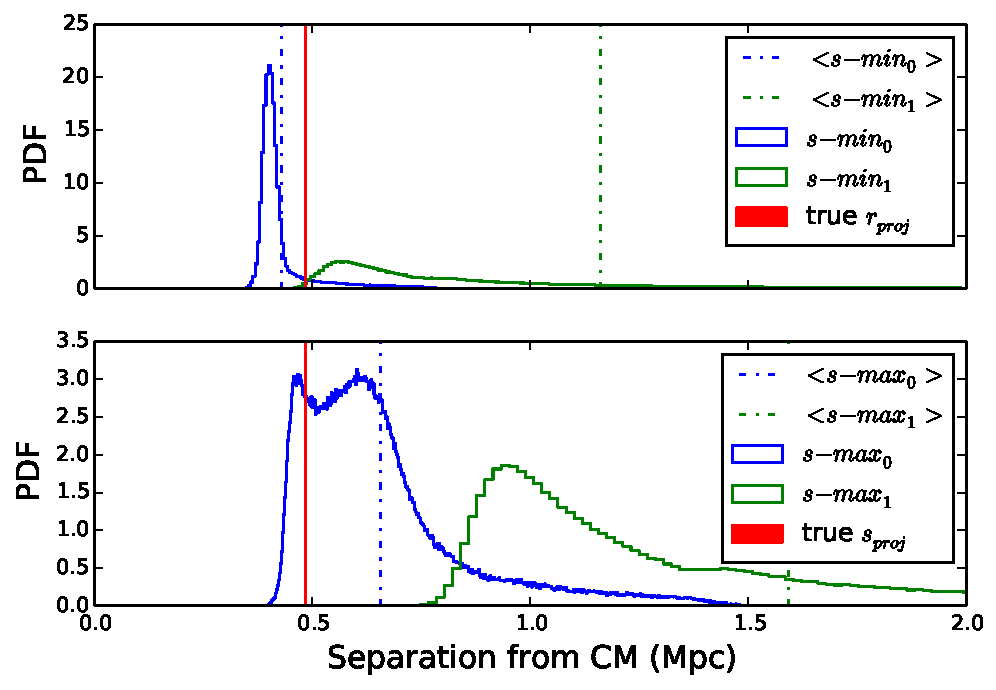
\includegraphics[width=\linewidth]{default_prior_bounds.pdf}
	\caption{Comparison of the observed position of the relic with the
	predicted position from the two simulated merger scenarios, with
	default prior applied to the PDFs.
	\label{fig: polarprior_bounds}}
\end{figure}




\bsp 
\label{lastpage} 

\end{document}
